\section{Aplikačná doména : Rakovina prsníka}

\subsection{Stavba prsníka}
\hspace{10mm}Ženský prsník sa skladá zväčša zo žľazového tkaniva a tuku, pričom jeho primárnou funkciou je tvorba materského mlieka pre výživu. Mliekotvorný bunkový systém sa skladá z mliekotvorných žľazových lalôčikov (lobuly), pričom tie sú spojené pomocou mliekovodov, ktoré sú prepojené do prsníkovej bradavky, v ktorej prúdi mlieko zo žliaz. Žľazy a mliekovody sú obalené tukom, ktoré určujú prsníku tvar a mäkkosť. Ich hlavnou úlohou je predovšetkým chrániť vnútornú štruktúru prsníka. Prsník neobsahuje žiadne svaly, ale je upnutý na veľkom prsnom svale (musculus pectoralis major), ktorý sa rozprestiera od plecového kĺbu ku kľúčnej kosti a odtiaľ až po hrudnú kosť. Po celom prsníku sa nachádzajú krvné cievy, ktoré dodávajú tkanivu hormóny a výživné látky. Táto sieť krvných ciev sa počas menštruácie, tehotenstva a sexuálneho vzrušenia napĺňa a spevňuje prsník. 

\begin{figure}[h!]
\begin{centering}
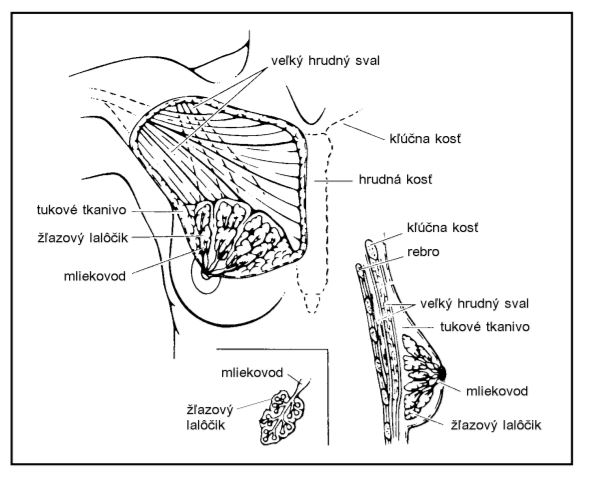
\includegraphics[width=15cm]{assets/images/242_1.JPG}
\par\end{centering}
\caption{Anatómia prsníka. \label{fig:dynabook}\cite{RAKOVINA-PRSNIKA}}
\end{figure}

\subsection{Lymfatický systém }
\hspace{10mm}Prsník obsahuje lymfatické cievy a lymfatické uzliny, teda lymfatický systém, ktorý zabezpečuje obrannú (imunitnú) úlohu v tele. Lymfatické uzliny slúžia ako filtračné stanice. Vďaka veľkému obsahu bielkovín dokážu zachytávať cudzie látky, organizmy,  ako sú baktérie, vírusy, nádorové bunky a mnoho iného. Počas života sa prsník nachádza v cykloch, pri ktorých sa opakovane vytvárajú uzlíky, pričom ich obsah nie je jednotný. Uzlíky sú z malých cýst a spojivového tkaniva, to sa nazýva fibrocystická mastopatopatia. Nezhubné uzlíky sa od zhubných (malígnych nádorov) dajú jednoducho rozlíšiť a to tak, že nezhubné uzlíky sa pred menštruáciou zväčšia a následne znova zmenšia. Tento cyklus môže u žien pretrvať aj po menopauze a to kvôli liekom s vysokým obsahom estrogénu alebo pokiaľ nadobličky stále produkujú pohlavné hormóny. V lymfatických cievach sa  z prsníka vyplavujú nečistoty, pričom časti ostávajú v lymfatických uzlíkoch. 


\subsection{Rizikové faktory vzniku rakoviny}
\hspace{10mm}Pri rakovine prsníka, tak ako pri väčšine druhov rakovín, nie sú presne určené príčiny vzniku, no vďaka štatistickým údajom sú zistené niektoré rizikové faktory, pomocou ktorých vieme znížiť pravdepodobnosť výskytu rakoviny. Sú to genetické faktory, napríklad, ak dvaja najbližší príbuzní mali rakovinu prsníka, potom má osoba asi 50\% šancu, že ju bude mať. Ďalším faktorom môže byť zlá životospráva (pokiaľ sa osoba stravovala výrazne tukmi či alkoholom)  a obezita. Rozhodujúcim faktorom je i vek, v ktorom mala žena prvú menštruáciu či  vek nástupu menopauzy. Podstatný je aj obsah hormónov. Rizikovými sú tiež ženy, ktoré rodili až po tridsiatke alebo ktoré nerodili vôbec.

\subsection{Diagnostika rakoviny prsníka}
\hspace{10mm}Diagnostika rakoviny prsníka spočíva v tom, že osoba buď príde na pravidelnú kontrolu, alebo si z vlastnej iniciatívy objaví hrčku v prsníku. Doktor následne vykoná palpačné vyšetrenie, podrobné prehmatanie prsníka, pričom sa zistí stav prvotného náleziska nádoru. Potom sa vykoná aj prezretie druhotného náleziska v podpazuší a nad kľúčnou kosťou. Druhým  krokom  diagnostiky je mamografia, čo je špeciálne röntgenové vyšetrenie, ktoré jasne ukáže, či pacient má rakovinu prsníka. Iným  krokom môže byť sonografia, pri ktorom sa zobrazujú aj iné orgány, ako sú pečeň, lymfatické uzliny, obličky a slezina. Toto vyšetrenie je bezpečnejšie, keďže sa robí pomocou ultrazvuku, tak nedochádza k žiadnemu ožarovaniu, aj keď pri mamografii vďaka moderným prístrojom je toto ožiarenie minimálne. U mladých žien doktori preferujú skôr sonografiu ako mamografiu. Pokiaľ boli doterajšie testy pozitívne, vykoná sa biopsia prsníka, teda zoberie sa tkanivo na mikroskopickú (histologickú) analýzu. Toto vyšetrenie je najpresnejšie zo všetkých, samozrejme, je to bezpečné. \cite{RAKOVINA-PRSNIKA}

\subsection{Podrobný opis témy a histologických dát} \label{HE2protein}
\hspace{10mm}Podľa súčasných smerníc sa musí ľudský receptor epidermálneho rastového faktora 2 (HER2) rutinne testovať spolu s receptormi estrogénu a progesterónu u všetkých pacientov s invazívnou rakovinou prsníka a ich metastázami. HER2 je transmembránový proteínový receptor s tyrozínkinázovou aktivitou. Tento receptor je amplifikovaný alebo nadmerne exprimovaný približne v 15 až 20\% v rakovine prsníka. Nadmerná expresia alebo amplifikácia HER2 bola spojená s agresívnym správaním rakoviny, pričom s vysokou pravdepodobnosťou na liečbu tejto rakoviny je cielená terapia na HER2. Mnoho klinických štúdií preukázalo, že liečba zameraná na HER2 podávaná počas alebo po chemoterapii, vedie k významnému zlepšeniu vyliečenia, teda k úplnému zbaveniu sa rakoviny a prežitia pacientov s rakovinou prsníka, ale len u pacientov so zvýšenou amplifikáciou alebo nadmernou expresiou HER2. V dôsledku toho správna identifikácia HER2 pozitívneho BC vyberá pacientov, u ktorých sa očakáva, že budú mať prospech z cielenej liečby, čím sa HER2 stane užitočným ukazovateľom pre rozhodovanie o liečbe u pacientov s rakovinou prsníka. Vo väčšine laboratórií začína hodnotenie HER2 analýzou proteínovej expresie pomocou imunohistochémie (IHC), ktorá vedie k nasledujúcim scenárom: negatívne, nejednoznačné, pozitívne a neurčité. Ak je výsledok IHC nejednoznačný alebo neurčitý, malo by sa vykonať reflexné testovanie pomocou in situ hybridizačných (ISH) testov na vyhodnotenie amplifikácie HER2. HER2 rakovina prsníka  je spojený s určitými morfologickými znakmi, ako je vysoký histologický stupeň, tak pri invazívnych  ako aj in situ léziách.
 \cite{ECDP2020}